\documentclass{beamer}
\usepackage{listings}
\usepackage{csvsimple}
\usepackage{listings}
\usepackage[utf8]{inputenc}
\lstdefinelanguage{scala}{
  morekeywords={abstract,case,catch,class,def,%
    do,else,extends,false,final,finally,%
    for,if,implicit,import,match,mixin,%
    new,null,object,override,package,%
    private,protected,requires,return,sealed,%
    super,this,throw,trait,true,try,%
    type,val,var,while,with,yield},
  otherkeywords={=>,<-,<\%,<:,>:,\#,@},
  sensitive=true,
  morecomment=[l]{//},
  morecomment=[n]{/*}{*/},
  morestring=[b]",
  morestring=[b]',
  morestring=[b]"""
}

\usepackage{color}
\definecolor{dkgreen}{rgb}{0,0.6,0}
\definecolor{gray}{rgb}{0.5,0.5,0.5}
\definecolor{mauve}{rgb}{0.58,0,0.82}

\lstset{frame=tb,
  language=scala,
  aboveskip=3mm,
  belowskip=3mm,
  showstringspaces=false,
  columns=flexible,
  basicstyle={\small\ttfamily},
  numbers=none,
  numberstyle=\tiny\color{gray},
  keywordstyle=\color{blue},
  commentstyle=\color{dkgreen},
  stringstyle=\color{mauve},
  frame=single,
  breaklines=true,
  breakatwhitespace=true
  tabsize=3
}



\lstdefinelanguage{VHDL}{
   morekeywords={
     library,use,all,entity,is,port,in,out,end,architecture,of,
     begin,and,
     LIBRARY,USE,ALL,ENTITY,IS,PORT,IN,OUT,END,ARCHITECTURE,OF,GENERIC,
     BEGIN,AND,SIGNAL,MAP,ATTRIBUTE,DOWNTO,GENERATE,FOR,CONSTANT,COMPONENT
   },
   morecomment=[l]--
}
\usepackage{xcolor}
\colorlet{keyword}{blue!100!black!80}
\colorlet{comment}{green!90!black!90}
\lstdefinestyle{vhdl}{
   language     = VHDL,
   basicstyle   = \ttfamily,
   keywordstyle = \color{keyword}\bfseries,
   commentstyle = \color{comment}
}




\begin{document}
    \section{VHDL}

    \begin{frame}[fragile]
    \frametitle{Micropipeline: Delay}
    \begin{lstlisting}
    room.audience.map(p => self.greet(p))
    \end{lstlisting}
    \end{frame}


    \begin{frame}[fragile]
        \frametitle{Package: delayPack}
        \begin{lstlisting}[style=vhdl,basicstyle=\ttfamily\small]
package delayPack is 
    COMPONENT n_delay 
              GENERIC (n : positive := 10);
              PORT (    n_del_in  : IN   std_logic;
                    n_del_out : OUT  std_logic);
    end COMPONENT;

    COMPONENT delay
              PORT (    del_in  : IN   std_logic;
                    del_out : OUT  std_logic); 
    end COMPONENT;
    
    CONSTANT delayTime: time;
end delayPack;

package body delayPack is
    CONSTANT delayTime : time := 1 ns;
end delayPack;

        \end{lstlisting}
    \end{frame}

    \begin{frame}[fragile]
        \frametitle{Entity}
        \begin{lstlisting}[style=vhdl]
ENTITY n_delay IS
GENERIC (n : positive := 10);
   PORT (n_del_in  :       IN     std_logic;
        n_del_out :       OUT    std_logic);
END n_delay;
        \end{lstlisting}
    \end{frame}

\begin{frame}[fragile]
        \frametitle{Architektur: Funktionale Simulation}
        \begin{lstlisting}[style=vhdl]
ARCHITECTURE timesim OF n_delay IS

SIGNAL intsig_delay : std_logic_vector(
    n DOWNTO 0);

begin
    gen_delays:
     FOR i IN (n) DOWNTO 1 GENERATE
    delay_instance: delay 
      PORT MAP (
          del_in  => intsig_delay(i),
          del_out => intsig_delay(i-1) 
          );
    end generate gen_delays;
    intsig_delay(n) <= n_del_in;
    n_del_out <= intsig_delay(0);
end timesim;
    \end{lstlisting}
\end{frame}

\begin{frame}[fragile]
        \frametitle{Architektur: Funktionale Simulation}
        \begin{lstlisting}[style=vhdl]
ENTITY delay IS
    PORT (    del_in  : IN  std_logic;
            del_out : OUT std_logic);
end delay;

ARCHITECTURE arch OF delay IS
begin
    del_out <= del_in AFTER delayTime;
END arch;
    \end{lstlisting}
\end{frame}




\begin{frame}[fragile]
        \frametitle{Testbench}
        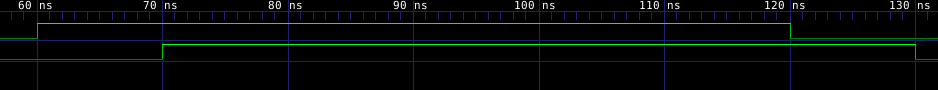
\includegraphics[width=\textwidth]{n_delay_func_sim1.png}
        \begin{lstlisting}[style=vhdl]
ARCHITECTURE arch of func_tb is 
SIGNAL in_sig, out_sig : std_logic;

BEGIN
  delay_instance : n_delay
    PORT MAP (in_sig, out_sig);

    in_sig <= '0',
              '1' after 60 ns,
              '0' after 120 ns;
END arch;
        \end{lstlisting}
\end{frame}


\begin{frame}[fragile]
    \frametitle{Synthetisierbare Architektur}
    Problem!
    \begin{itemize}
        \item Verzögerung mit \texttt{after} wird wegoptimiert!
    \end{itemize}
    Idee!
    \begin{itemize}
        \item Verwende anstatt dem für die funktionale Simulation erstellten \texttt{delay} eine Lookup-Table (LUT).
        \item Wähle die Funktion \texttt{Buffer}, welche nach kurzer Verzögerung das Eingabe - Signal weiterleitet.
    \end{itemize}
\end{frame}

\begin{frame}[fragile]
    \frametitle{Synthetisierbare Architektur}
    Es funktioniert!
    \begin{itemize}
        \item Verzögerung wird nicht mehr optimiert.
    \end{itemize}
    Aber!
    \begin{itemize}
        \item Jeder Synthetisierungsvorgang erzeugt andere Verzögerungszeiten! $\rightarrow$ PFUI!
        \item Die Platzierung der Lookup-Tables auf dem Board ist nicht deterministisch.
        \item Unterschiede in der Länge der Verbindungsleitungen erzeugen unterschiedliche Verzögerungszeiten.
    \end{itemize}
    Lösung!
    \begin{itemize}
        \item Relative Location Constraints (\texttt{RLOC})!
        \item Erzwinge relative Lage der Komponenten.
    \end{itemize}
\end{frame}





    \begin{frame}[fragile]
        \frametitle{Synthetisierbare Architektur}
        \begin{lstlisting}[style=vhdl]
ARCHITECTURE deterministic OF n_delay IS

SIGNAL intsig_delay : std_logic_vector(
    n DOWNTO 0);
ATTRIBUTE RLOC : string;

ATTRIBUTE syn_hier : string;
ATTRIBUTE syn_hier OF deterministic : 
    ARCHITECTURE IS "hard";

ATTRIBUTE xc_use_xmodule: boolean;
ATTRIBUTE xc_use_keep_hierarchy OF deterministic : 
    ARCHITECTURE IS true;

\end{lstlisting}
\end{frame}

    \begin{frame}[fragile]
        \frametitle{Synthetisierbare Architektur}
        \begin{lstlisting}[style=vhdl]
BEGIN n_delay:
FOR i IN (n) DOWNTO 1 GENERATE
  CONSTANT param : natural  := 
      ((n-i)) mod 2;
  CONSTANT row : natural    := 
      ((n-i)/4) mod 2;
  CONSTANT column : natural := 
      (n-i)/4 + (param - row);
  CONSTANT rloc_str : string := 
      "X" & itoa(row) & "Y" & itoa(column);
    
  ATTRIBUTE RLOC of lut_instance : 
      LABEL IS rloc_str;
        \end{lstlisting}
rloc\_str: X0Y0,X0Y1,X0Y0,X0Y1,X1Y0,X1Y1,...
\end{frame}
    \begin{frame}[fragile]
        \frametitle{Synthetisierbare Architektur}
        \begin{lstlisting}[style=vhdl]
BEGIN

  lut_instance: LUT1
    GENERIC MAP (
      INIT => "0000000000000010"
      )   -- Buffer 10
        
    PORT MAP (
      O  => intsig_delay(i),
      I0 => intsig_delay(i-1)
      );

END GENERATE;
intsig_delay(0) <= n_del_in;
n_del_out <= intsig_delay(n);
END deterministic;
        \end{lstlisting}
\end{frame}






\frame{
   \frametitle{Timing - Simulation}
   %\csvautotabular{times.csv}
   \centering
   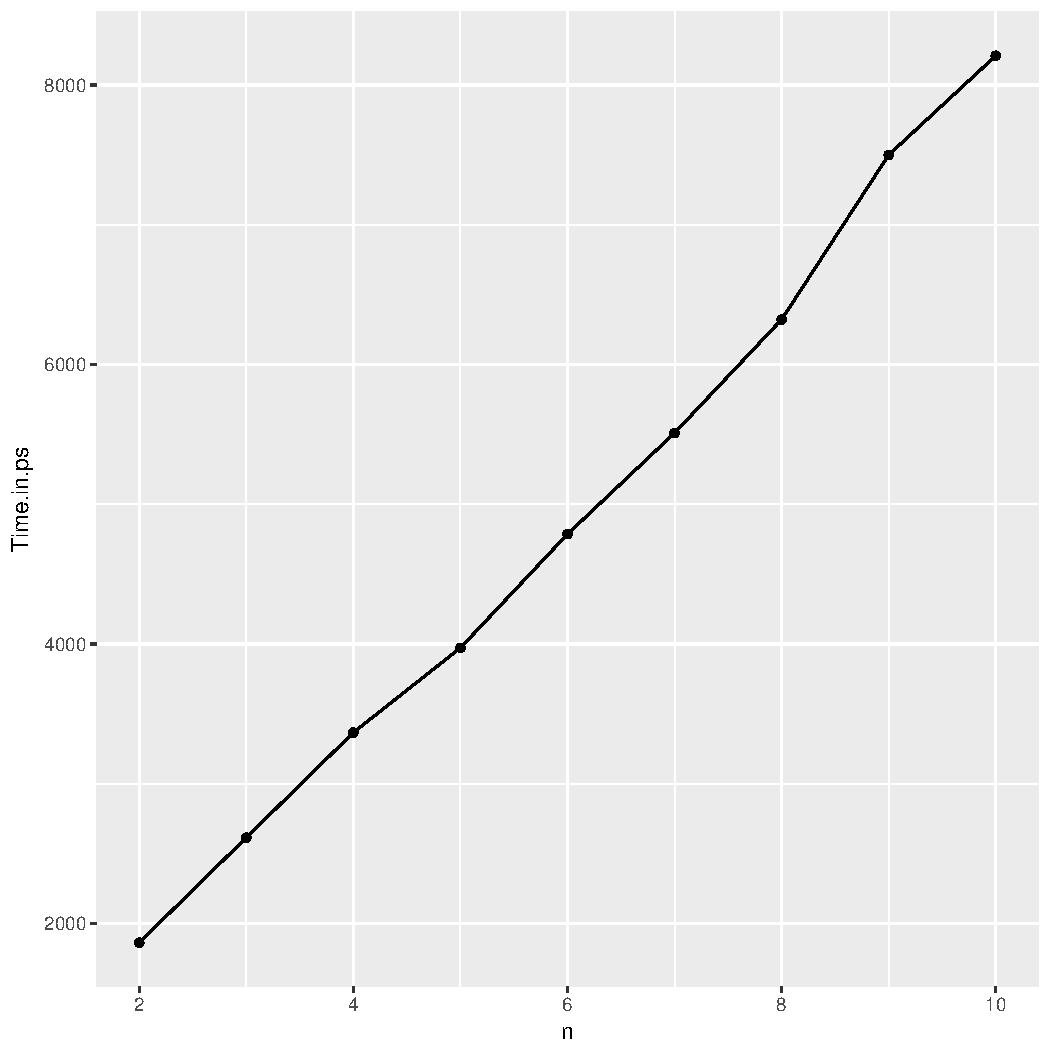
\includegraphics[width=0.8\textwidth,height=0.8\textheight]{func_sim.pdf}}
%The following is a list of a few of the functions you can perform on your designs in the FPGA Editor.
%    Place and route critical components before running the automatic place and route tools.
%    Finish placement and routing if the routing program does not completely route your design.
%    Add probes to your design to examine the signal states of the targeted device. Probes are used to route the value of internal nets to an IOB for analysis during the debugging of a device.
%    Cross-probe your design with Timing Analyzer.
%    Run the BitGen program and download the resulting BIT file to the targeted device.
%    View and change the nets connected to the capture units of a ChipScope ILA core in your design.
%    Use the ILA command to write a ChipScope Import document (.cdc) file
%    Create an entire design by hand (advanced users). 
    \frame{
        \frametitle{FPGA-Editor}
            \begin{enumerate}
                \item Manuelles Platzieren und Verbinden von Elementen
                \item Sondieren von internen Zuständen an beliebigen Stellen der Schaltung
                \item Downloaden von generierten Bit-Dateien auf das Gerät
                \item Kompletter Designvorgang von Hand möglich.
            \end{enumerate}

    }

    \frame{
        \frametitle{FPGA-Editor}
        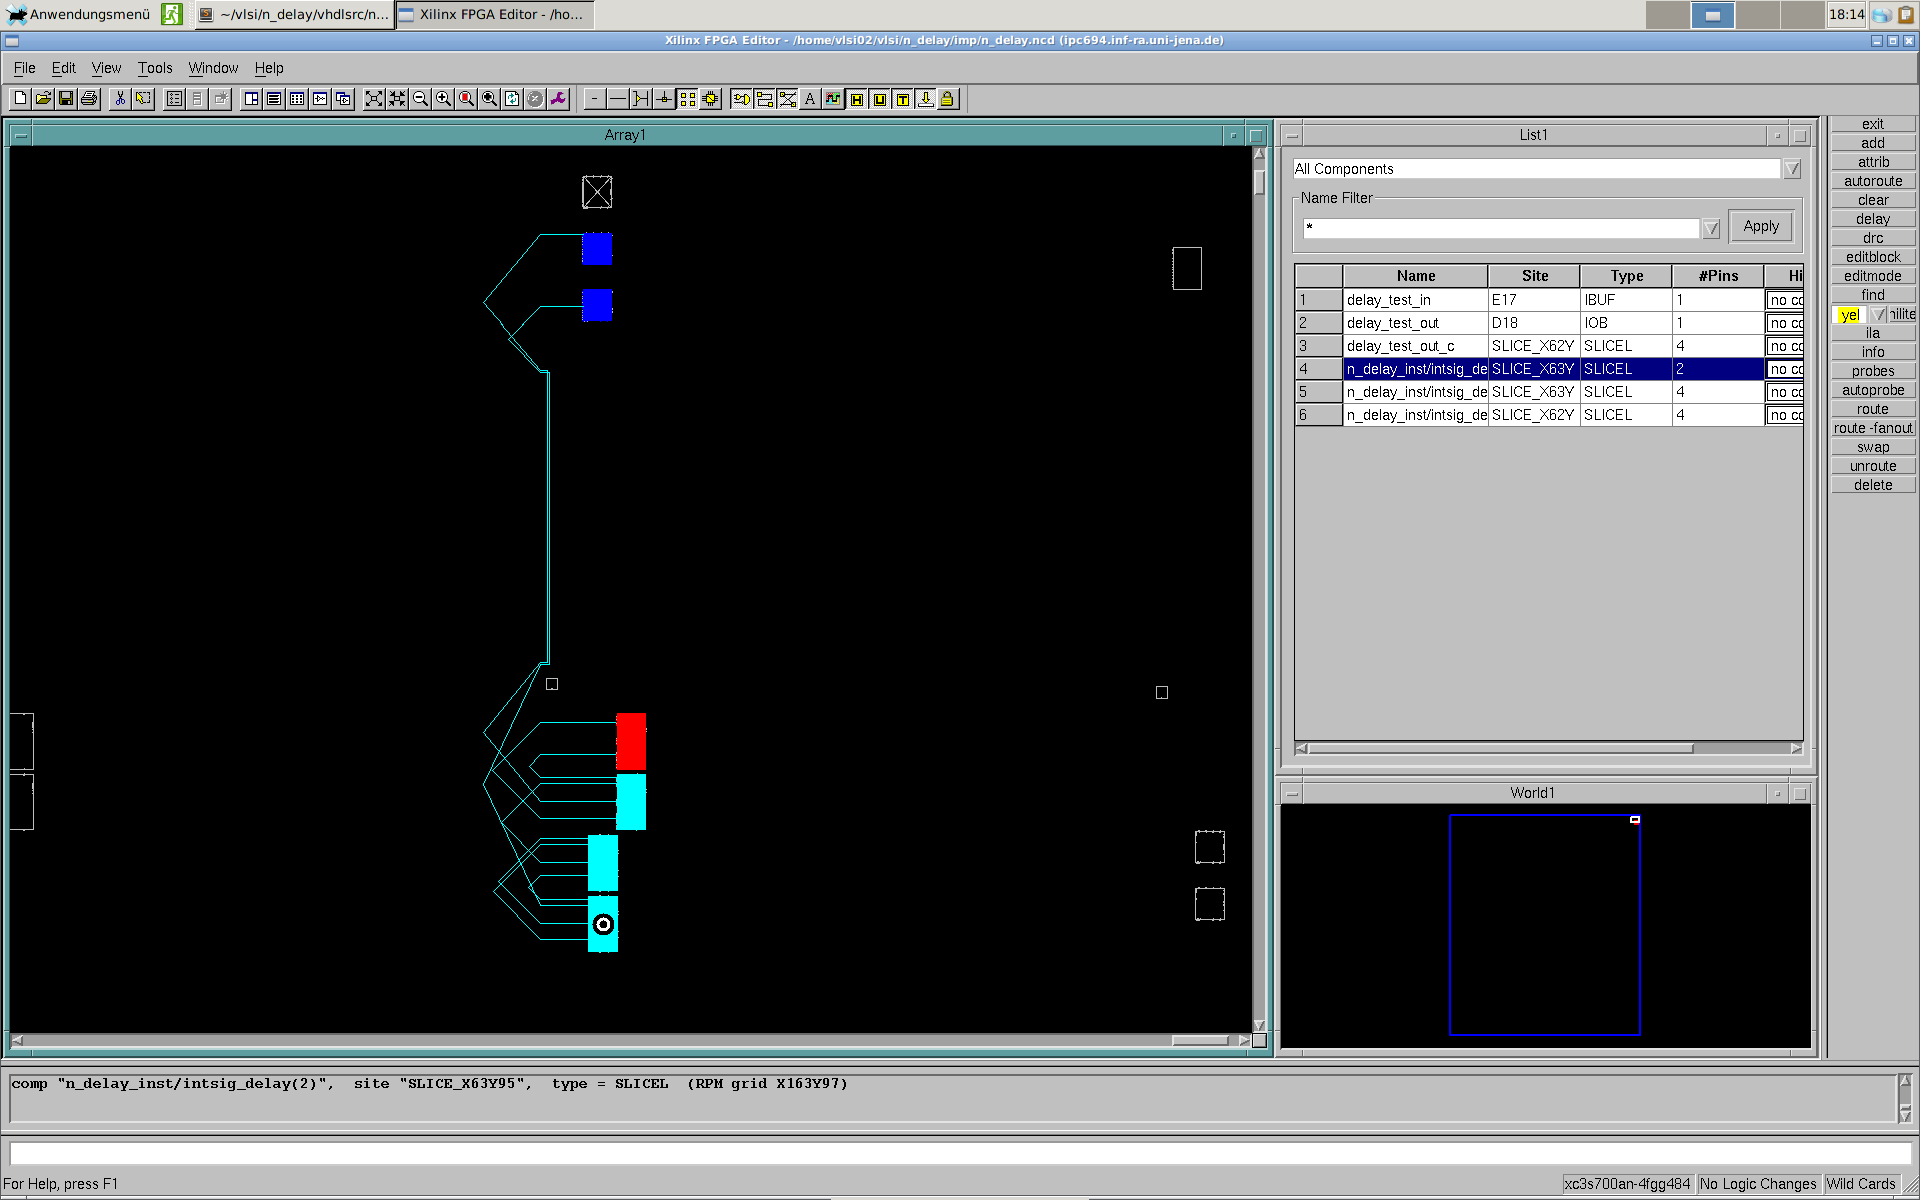
\includegraphics[width=\textwidth]{editor_overview.png}
    }

    \frame{
        \frametitle{FPGA-Editor}
        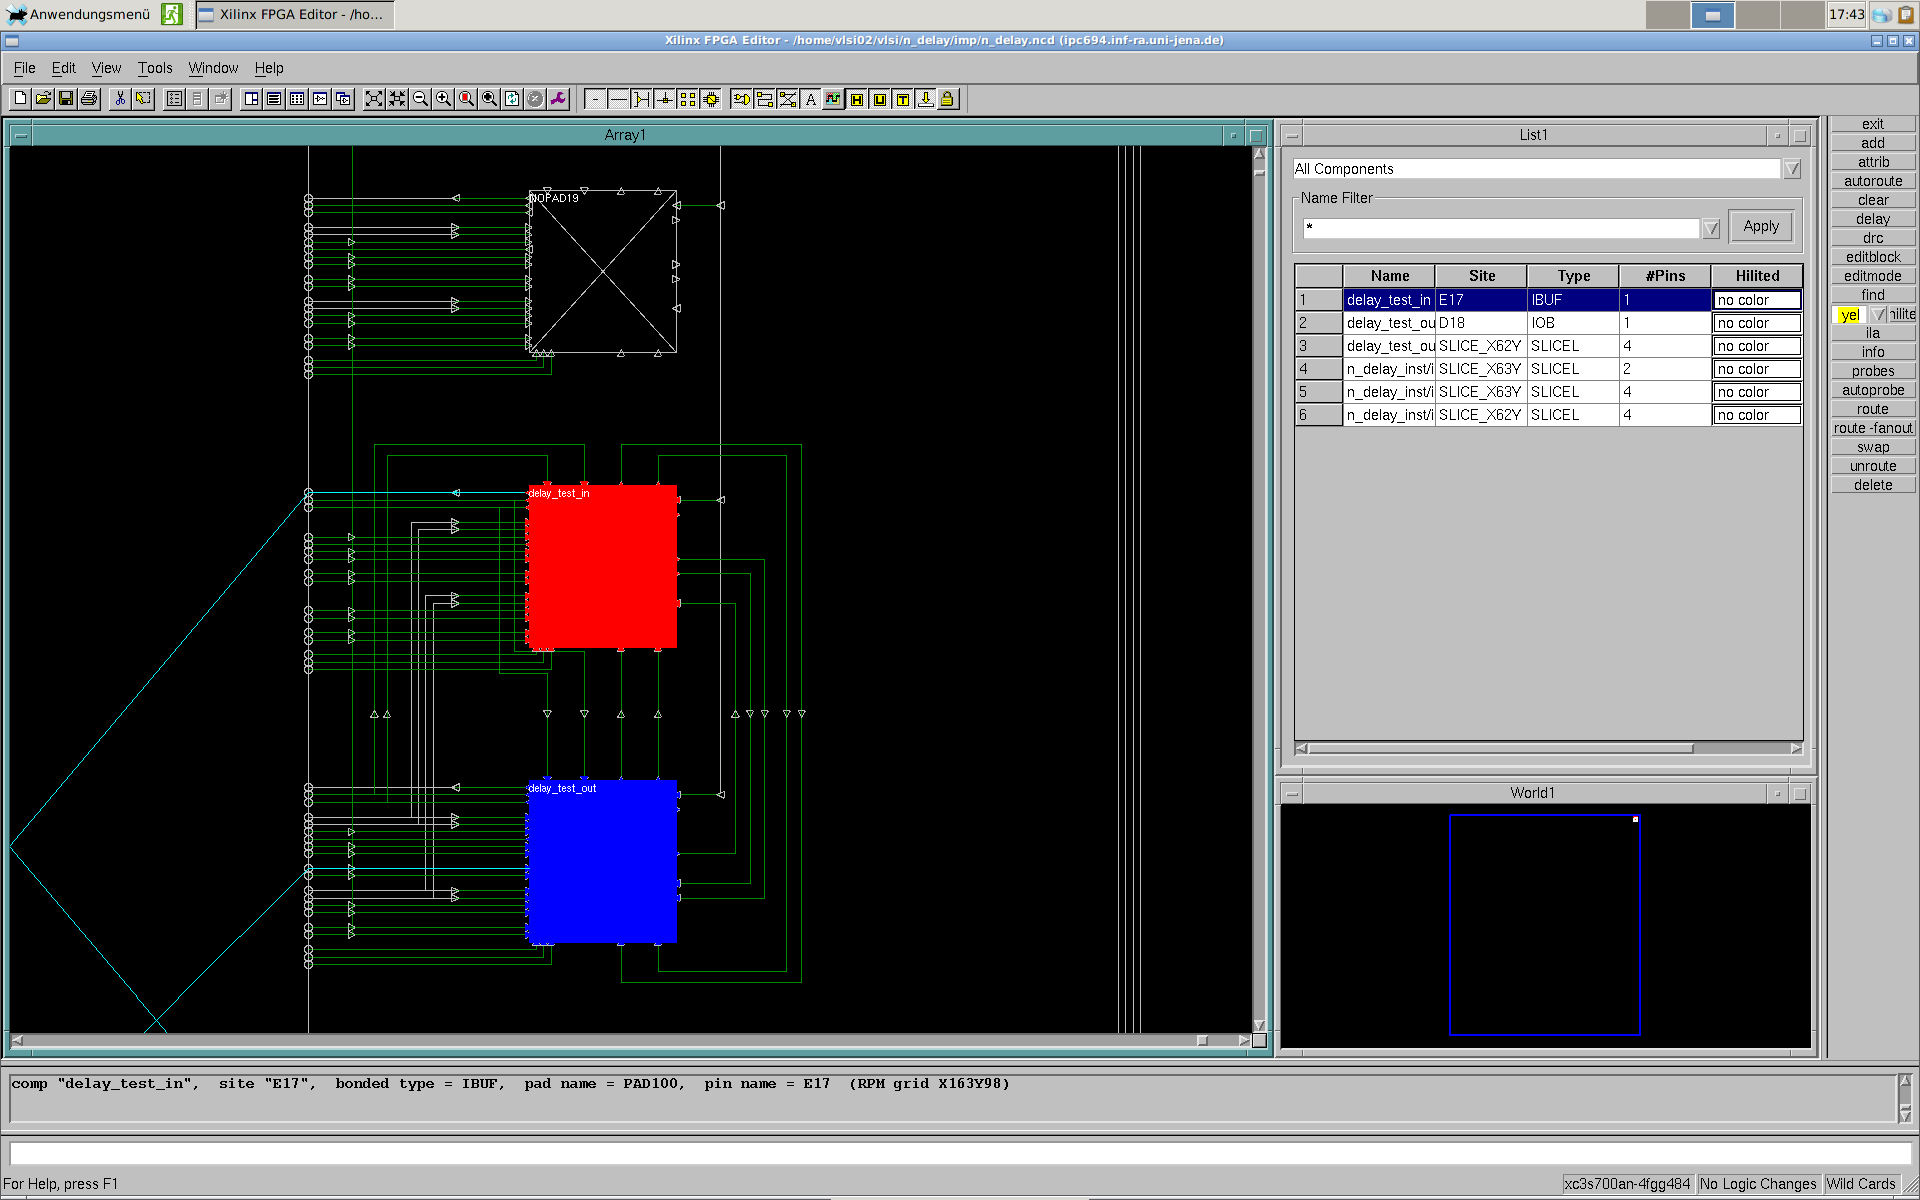
\includegraphics[width=\textwidth]{editor1.png}
    }

     \frame{
        \frametitle{FPGA-Editor}
        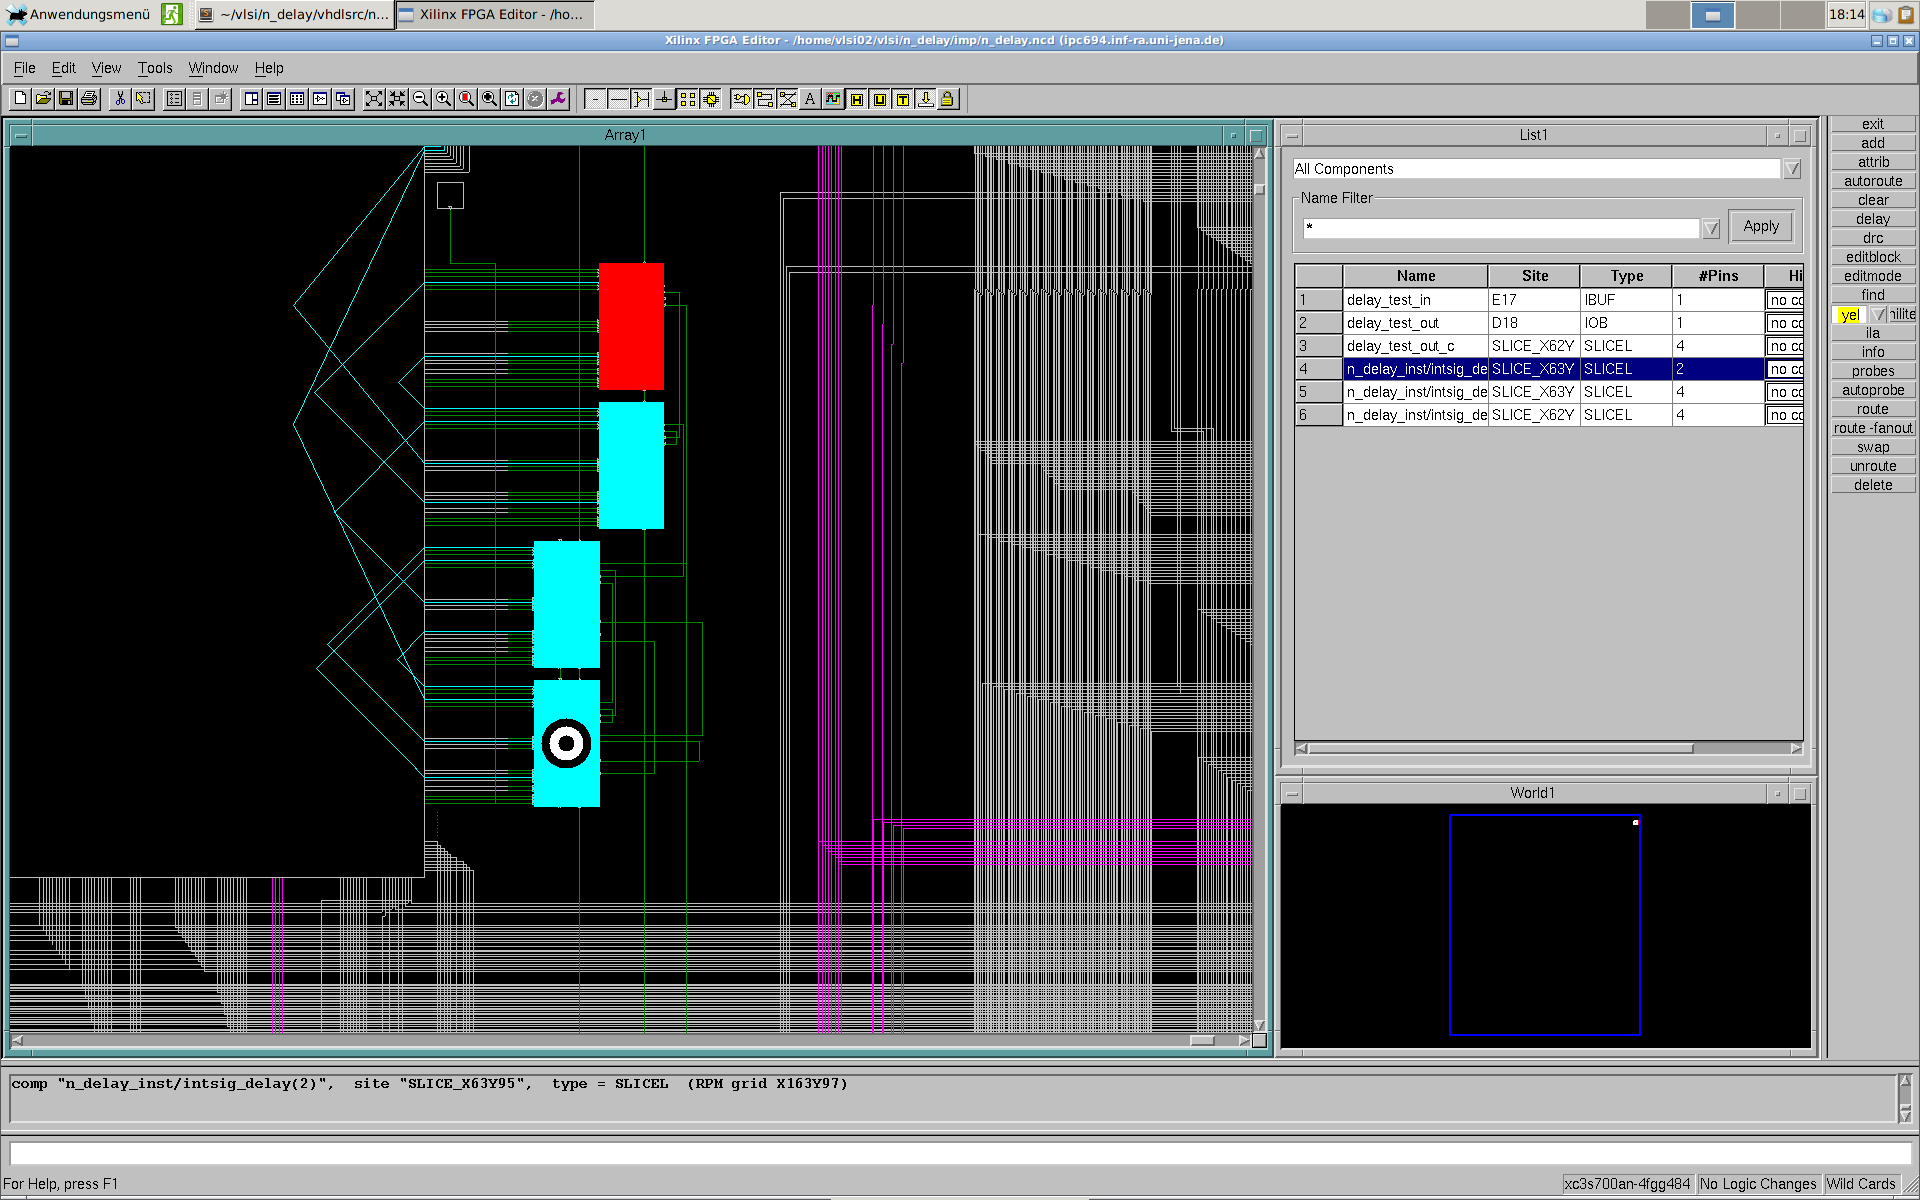
\includegraphics[width=\textwidth]{editor_fine.png}
    }

     \frame{
        \frametitle{FPGA-Editor}
        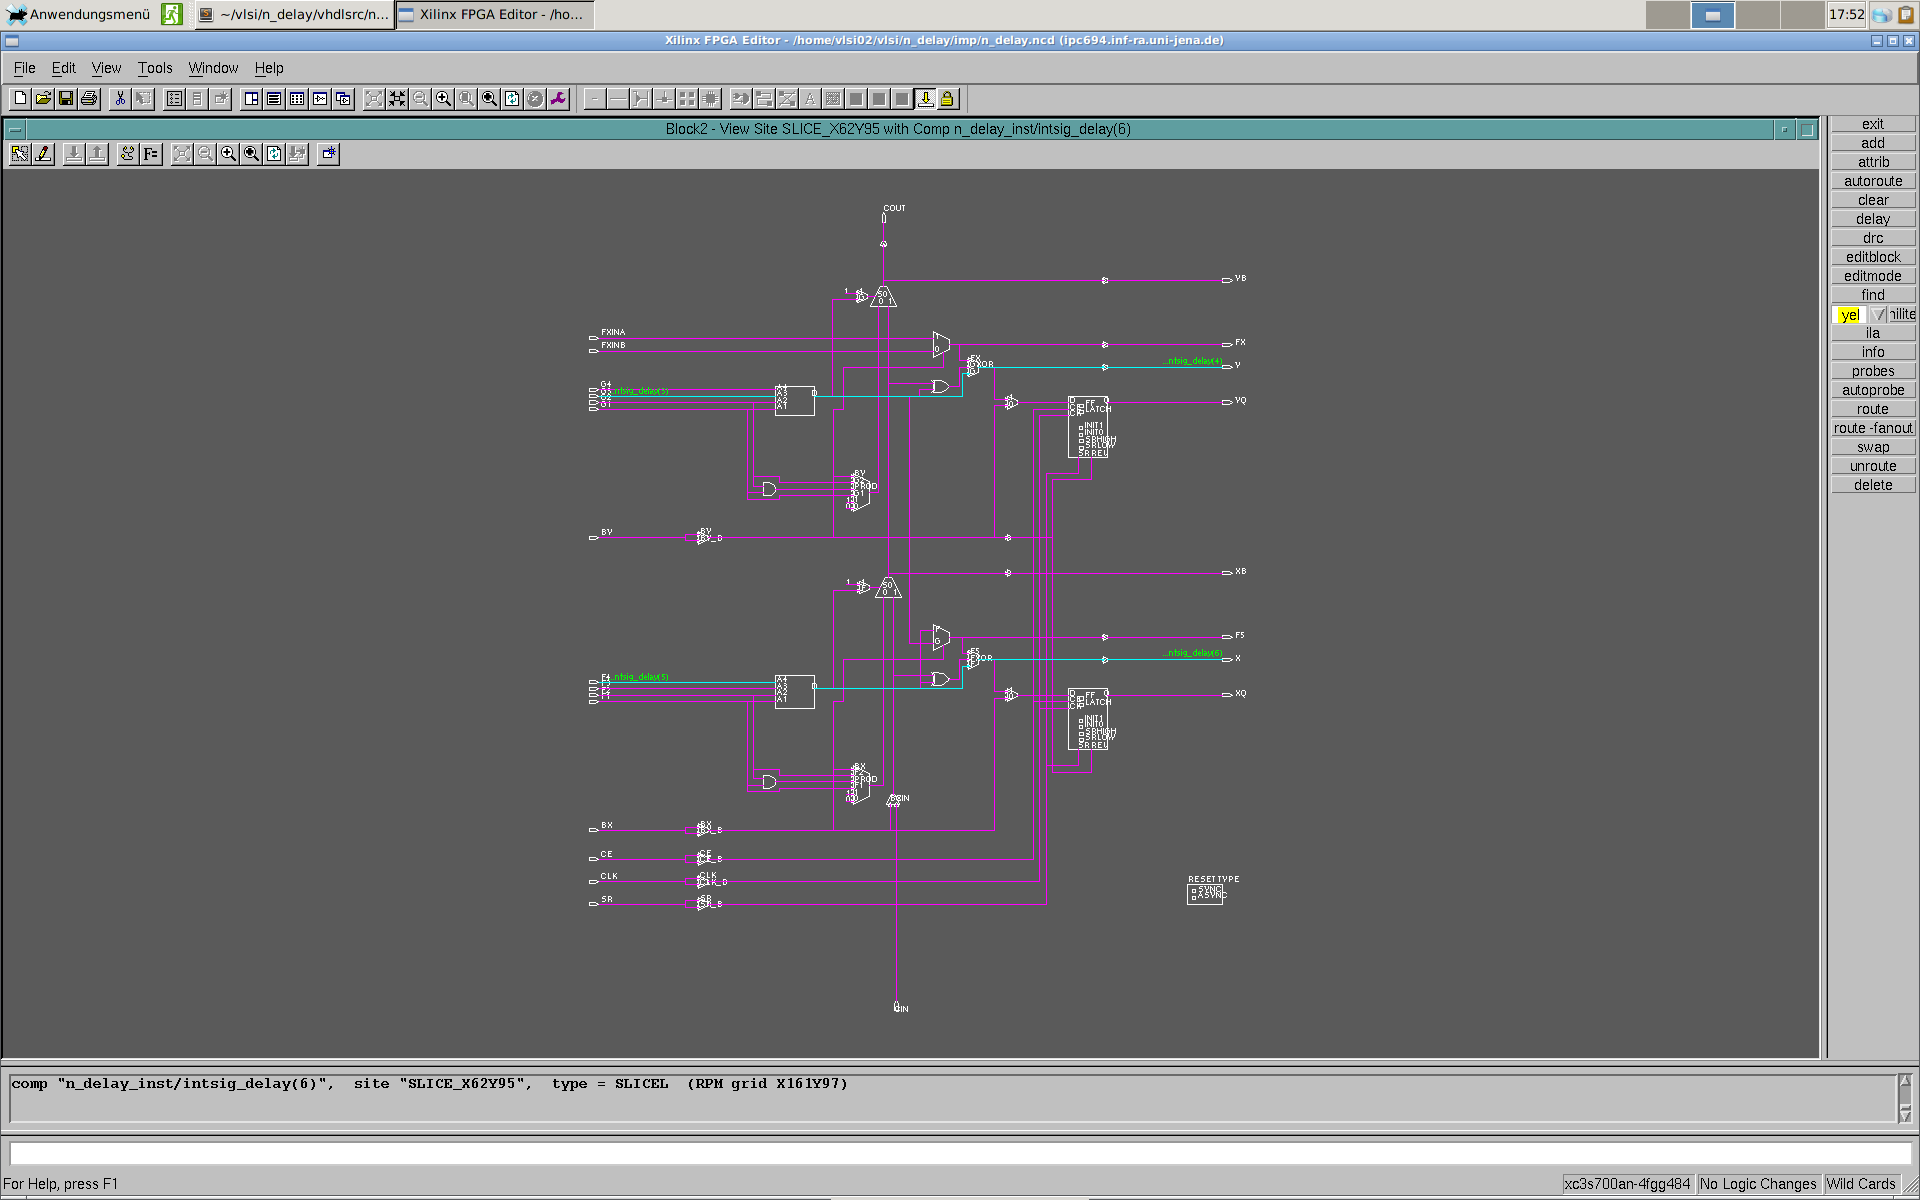
\includegraphics[width=\textwidth]{editor_slice.png}
    }

\end{document}
